\documentclass[border=4pt]{standalone}
\usepackage{tikz}
\usetikzlibrary{arrows.meta,positioning,calc,fit,backgrounds,patterns,shapes.geometric}
\usepackage{amsmath,amssymb}
\usepackage{mathptmx}
\definecolor{lost}{HTML}{C2362D}
\definecolor{kept}{HTML}{17875A}
\definecolor{evid}{HTML}{3056D3}
\definecolor{ink}{HTML}{1D1D1F}
\definecolor{muted}{HTML}{6E6E73}
\tikzset{
  box/.style={draw=ink!70, rounded corners=2pt, align=center, fill=white, inner sep=4pt, font=\footnotesize},
  arr/.style={-{Stealth[length=2mm]}, draw=ink!70, line width=0.6pt},
  grp/.style={draw=muted!60, dashed, rounded corners=4pt, inner sep=7pt},
  lossbox/.style={draw=lost!80, fill=lost!6, text=lost!85!black, rounded corners=2pt, align=left, font=\footnotesize, inner sep=4pt},
  fixbox/.style={draw=kept!80, fill=kept!7, text=kept!65!black, rounded corners=2pt, align=left, font=\footnotesize, inner sep=4pt},
  dec/.style={diamond, aspect=2.2, draw=ink!70, fill=evid!6, align=center, font=\footnotesize, inner sep=1.5pt},
  lbl/.style={font=\footnotesize\bfseries, text=ink},
}

\begin{document}
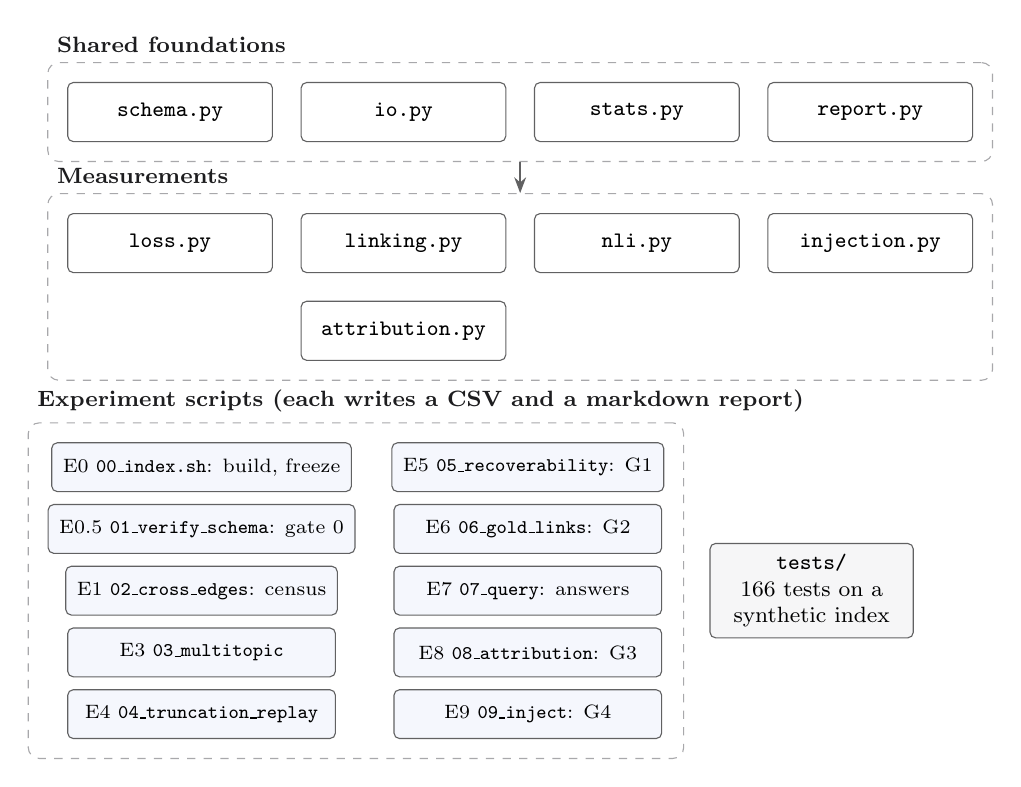
\begin{tikzpicture}[node distance=0.35cm]
\tikzset{m/.style={box, minimum width=2.6cm, minimum height=0.75cm}, s/.style={box, minimum width=3.4cm, minimum height=0.62cm, fill=evid!5, font=\scriptsize}}
\node[m] (schema) {\texttt{schema.py}};
\node[m, right=of schema] (io) {\texttt{io.py}};
\node[m, right=of io] (stats) {\texttt{stats.py}};
\node[m, right=of stats] (report) {\texttt{report.py}};
\node[m, below=0.9cm of schema] (loss) {\texttt{loss.py}};
\node[m, right=of loss] (linking) {\texttt{linking.py}};
\node[m, right=of linking] (nli) {\texttt{nli.py}};
\node[m, right=of nli] (inj) {\texttt{injection.py}};
\node[m, below=0.35cm of linking] (attr) {\texttt{attribution.py}};
\begin{scope}[on background layer]
\node[grp, fit=(schema)(io)(stats)(report), label={[lbl, anchor=south west]north west:Shared foundations}] (gA) {};
\node[grp, fit=(loss)(linking)(nli)(inj)(attr), label={[lbl, anchor=south west]north west:Measurements}] (gB) {};
\end{scope}
\draw[arr] (gA.south) -- (gB.north);
\node[s] (e0) at ($(loss.south |- attr.south)+(0.4,-1.35)$) {E0 \texttt{00\_index.sh}: build, freeze};
\node[s, below=0.15cm of e0] (e05) {E0.5 \texttt{01\_verify\_schema}: gate 0};
\node[s, below=0.15cm of e05] (e1) {E1 \texttt{02\_cross\_edges}: census};
\node[s, below=0.15cm of e1] (e3) {E3 \texttt{03\_multitopic}};
\node[s, below=0.15cm of e3] (e4) {E4 \texttt{04\_truncation\_replay}};
\node[s, right=0.5cm of e0] (e5) {E5 \texttt{05\_recoverability}: G1};
\node[s, below=0.15cm of e5] (e6) {E6 \texttt{06\_gold\_links}: G2};
\node[s, below=0.15cm of e6] (e7) {E7 \texttt{07\_query}: answers};
\node[s, below=0.15cm of e7] (e8) {E8 \texttt{08\_attribution}: G3};
\node[s, below=0.15cm of e8] (e9) {E9 \texttt{09\_inject}: G4};
\begin{scope}[on background layer]
\node[grp, fit=(e0)(e05)(e1)(e3)(e4)(e5)(e6)(e7)(e8)(e9), label={[lbl, anchor=south west]north west:Experiment scripts (each writes a CSV and a markdown report)}] (gC) {};
\end{scope}
\node[m, right=0.6cm of e7, minimum width=2.4cm, text width=2.3cm, fill=muted!6] (tests) {\texttt{tests/}\\166 tests on a synthetic index};
\end{tikzpicture}
\end{document}
